\documentclass[UTF8]{ctexart}
\usepackage{amsmath}
\usepackage{geometry}
\geometry{left=2.54cm,right=2.54cm,top=3.09cm,bottom=3.09cm}
\usepackage{graphicx}
\usepackage{float}

\begin{document}
	对于两点边值问题:
	\begin{align*}
		\begin{split}
			\left\{
				\begin{array}{ll}
					-\frac{d^2 u}{dx^2}=x^2, &0<x<1\\
					u(0)=0,\quad u(1)=0
				\end{array}
			\right.
		\end{split}
	\end{align*}

	其Ritz变分问题为:
	\begin{align*}
		\begin{split}
			\left\{
			\begin{array}{lr}
				u\in K,\quad s.t.\\
				J(u)\leq J(w), \quad \forall w \in K
			\end{array}
			\right.
		\end{split}
	\end{align*}
	其中$J(u)=\frac{1}{2}D(u,u)-F(u)$,\quad
	$D(u,v)=\int_0^1 \frac{du}{dx} \frac{du}{dx} dx$,\quad
	$F(u)=\int_0^1 x^2 v dx$.
	~\\
	
	
	采用Ritz方法求解,并取$K=C_0^1[0,1]$,取基函数$\varphi_1,\varphi_2,...\varphi_N$,其中$\varphi_i=x^i(1-x)$。则该问题化简为:
	求解$Dc^0=F$,\newline
	其中$D\in R^{n*n},D_{ij}=D(\varphi_i,\varphi_j)$,$c^0\in R^n$,$F\in R^n,F_i=F(\varphi_i)$.\newline
	则近似解$u_N=\sum_{i=1}^{N}c^0_i \varphi_i$.
	~\\
	
	\textbf{1.求解$D$与$F$,解方程组$Dc^0=F$:}
		\begin{align*}
			D_{ij} &=D(x^i(1-x),x^j(1-x))\\
			&=\int_{0}^{1}[ix^{i-1}(1-x)-x^i][jx^{i-1}(1-x)-x^i]dx\\
			&=\frac{(i+1)(j+1)}{i+j+1}-\frac{i(j+1)+j(i+1)}{i+j}+\frac{ij}{i+j-1}\\
			&=\frac{ij}{(i+j+1)(i+j)(i+j-1)}
		\end{align*},
		\begin{align*}
			F_i &=F(x^i(1-x))\\
			&=\int_{0}^{1}x^{2+i}(1-x)dx\\
			&=\frac{1}{3+i}-\frac{1}{4+i}\\
			&=\frac{1}{(3+i)(4+i)}
		\end{align*}
	
		解方程组$Dc^0=F$,$u_N=\sum_{i=1}^{N}c^0_i \varphi_i$.
		~\\
			
	\textbf{2.估计误差:}
	
		已知方程精确解$u=\frac{x}{12}(1-x^3)$,令相对误差$e=\frac{\int_0^1 (u-u_N)^2dx}{\int_0^1u^2dx}
		=\frac{\int_0^1 [\frac{x}{12}(1-x^3)-\sum_{i=1}^{N}c^0_i x^i(1-x)]^2 dx}{\frac{1}{108}}$,由于N较大时,直接求解该积分较麻烦,因此采用数值方法:
		
		这里我采用Romberg算法,令$T_m^k$为二分k次,加速m次得到的梯形值,令$f=(u-u_N)^2$:\\
		$T_0^0=\frac{f(0)+f(1)}{2}$\\
		$h=\frac{1}{2^k}$\\
		$T_0^k=\frac{h}{2}[f(a)+2\sum_{i=1}^{2^k-1}f(x_i)+f(b)]=\frac{h}{2}[f(a)+2\sum_{i=1}^{2^k-1}f(\frac{i}{2^k})+f(b)]$\\
		$T_0^{k+1}=\frac{1}{2}T_0^{k}+\frac{h}{2}\sum_{i=0}^{2^k-1}f(x_{i+\frac{1}{2}})=\frac{1}{2}T_0^{k}+\frac{h}{2}\sum_{i=0}^{2^k-1}f(hi+\frac{h}{2})$\\
		$T_1^k=\frac{4}{3}T_{0}^{k+1}-\frac{1}{3}T_{0}^k$\\
		$e=T_1^k$\\
		将N从1开始增加至10,得到如下误差曲线:
		\begin{figure}[H]
			\centering
			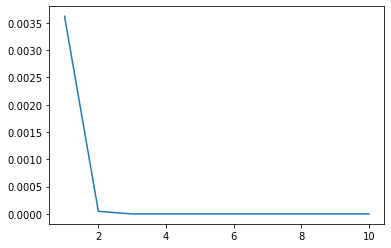
\includegraphics[width=0.5\textwidth]{err.png}
			\caption{$\epsilon=10^{-4}$误差图}
		\end{figure}
		故N取3时误差最小,约为$7*10^{-32}$,此时向量$c^0$的各项均为$\frac{0.25}{3}$,故近似解$u_N=\frac{x(1-x^3)}{12}$,与精确解相同
	
	
\end{document}
